\chapter{Metodologia}
\label{cap:Metodologia}

Neste capítulo serão apresentadas as duas estratégias propostas e desenvolvidas nesta dissertação para o PDP simplificado. A primeira trata de uma abordagem multi-objetiva utilizando dois AEMOs. Já a segunda visa aplicação da evolução gramatical  para gerar heurísticas de alto nível para um \textit{framework} hiper-heurístico intitulada EGHyPDP.


O problema PDP simplificado foi modelado utilizando a representação relativa, descrita na subseção \ref{subsubsection:modeloHP}, afim de codificar as possíveis estruturas de proteínas em vetores de inteiros. Segundo o estudo realizado por  \cite{krasnogor1999protein} esta representação possui um maior potencial em conduzir os algoritmos a resultados melhores. Cada gene do cromossomo especifica a direção que o amino ácido atual deve ser posicionado. Cada amino ácido é posicionado na direção codificada pelo respectivo gene em relação ao amino ácido anterior. O genes podem assumir apenas 3 valores:

\begin{itemize}
	\item 0 indica que o próximo amino ácido deve ser posicionado à direita do amino ácido anterior
	\item 1 indica que o próximo amino ácido deve ser posicionado à frente do amino ácido anterior
	\item 2 indica que o próximo aminoácido deve ser posicionado à esquerda do amino ácido anterior.
\end{itemize}

A Figura \ref{img:cromossomo} apresenta um exemplo de um cromossomo hipotético e a conformação gerada no \textit{grid} para o modelo HP-2D.


\begin{figure}[!htb]
	\centering
	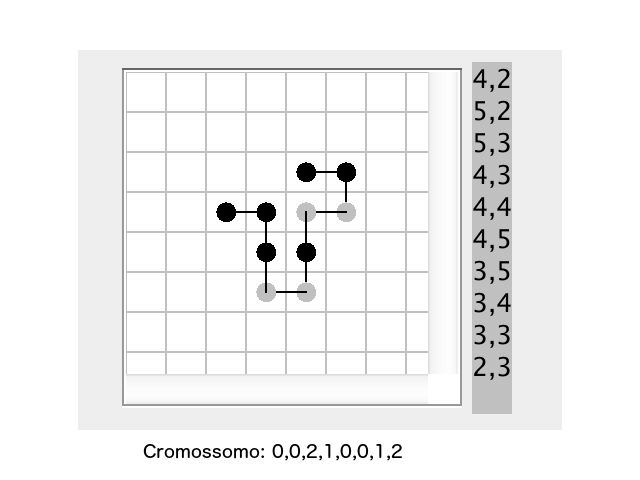
\includegraphics[scale=0.36]{Imagens/DecodedCromossome.png}
	\caption{Cromossomo decodificado que representa uma possível conformação para a cadeia HHPPHPPHHH}
	\label{img:cromossomo}
\end{figure}



Para ambas as abordagens o mesmo conjunto de heurísticas de baixo nível (operadores de cruzamento/mutação e busca locais) foi selecionado a partir dos estudos anteriores \cite{custodio2014multiple, custodio2004investigation, garza2012locality,benitez2015algoritmo}. O conjunto de heurísticas de baixo nível será descrito abaixo:

 \begin{itemize}
 	
 		\item \textit{Single Point Crossover} (1X): Este operador seleciona, de maneria aleatória, 1 ponto de cruzamento dividindo os indivíduos em 2 partes. Os genes entre as posições selecionadas são trocados entre os pais de modo a gerar dois novos filhos \cite{benitez2015algoritmo}.
 	
 	\item \textit{Two Points Crossover} (2X): Este operador seleciona, de maneria aleatória, 2 pontos de cruzamento dividindo os indivíduos em 3 partes. Os genes entre as posições selecionadas são trocados entre os pais de modo a gerar dois novos filhos \cite{benitez2015algoritmo}, conforme apresentado na figura \ref{fig:twopointscrossover}.
 	
 	
 	\begin{figure}[!htb]
 		\centering
 		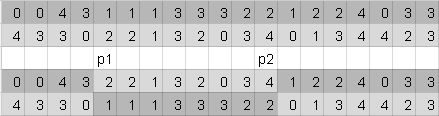
\includegraphics{Imagens/TwoPointsCrossover.png}
 		\caption{Exemplo de aplicação do operador 2x. \\Fonte Autoria Própria}
 		\label{fig:twopointscrossover}
 	\end{figure}
 	
 	
 	
 	
 	\item \textit{Multi Points Crossover} (MPX): Semelhante ao 2X porém com c pontos, baseado na função $c = int(n * 0.1)$, onde $n$ é o tamanho da sequência. O operador MPX é utilizado para promover diversidade estrutural realizando uma mescla randômica entre os pais. Embora, não tão radical quanto o \textit{Uniform  Crossover} \cite{sabar2015automatic}. Um exemplo de aplicação do operador MPX é apresentado na imagem \ref{fig:multipointscrossover}
 	
 	
 	\begin{figure}[!htb]
 		\centering
 		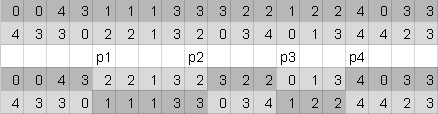
\includegraphics{Imagens/MultiPointsCrossover.png}
 		\caption{Exemplo de aplicação do operador MPX. \\Fonte Autoria Própria}
 		\label{fig:multipointscrossover}
 	\end{figure}
 	\item \textit{Segment Mutation} (SMUT): Altera um número aleatório (5 a 7) de genes consecutivos para direções distintas. Esta heurística introduz grandes mudanças na conformação, e tem uma grande probabilidade de criar colisões. Um mecanismo de reparação simples é aplicado no descendente gerado. A imagem \ref{fig:segmentMutation} apresenta um exemplo da aplicação do SMUT.
 	
 	\begin{figure}[!htb]
 		\centering
 		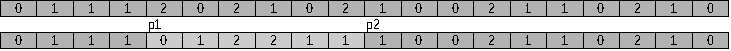
\includegraphics{Imagens/segmentMutation.png}
 		\caption{Exemplo de aplicação do operador SMUT. \\Fonte Autoria Própria}
 		\label{fig:segmentMutation}
 	\end{figure}
 	
 	
 	\item \textit {Exhaustive Search Mutation} (EMUT): Esta heurística seleciona um gene aleatório e testa todas as outras direções possíveis. Manterá a alteração que conseguir aumentar a qualidade da estrutura. O \textit{tradeoff} deste operador é demandar 4 avaliações de \textit{fitness}, há mais que as demais. Esta heurística tem grande potencial de melhorar o \textit{fitness} de uma estrutura. 
 	
 	
 	\item \textit{Local Move Operator} (LM): Esta heurística troca direções entre dois genes aleatórios consecutivos. Existem algumas condições para que esta heurística possa ser executada, por exemplo, as novas direções não podem criar movimentos redundantes. A figura \ref{fig:localMoveOperator} apresenta um exemplo da aplicação do operador LM. 
 	
 	
 	\begin{figure}[!htb]
 		\centering
 		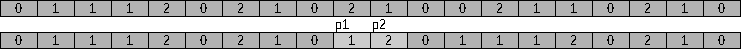
\includegraphics{Imagens/LocalMoveOperator.png}
 		\caption{Exemplo de aplicação do operador LM. \\Fonte Autoria Própria}
 		\label{fig:localMoveOperator}
 	\end{figure}
 	
 	
 	\item \textit{Loop Move Operator} (LPM): Da mesma maneira que a heurística LM, esta heurística troca direções entre dois genes que estão a 5 genes de distância na sequência. A figura  \ref{fig:loopMoveOperator} apresenta um exemplo da aplicação do operador LPM.
 	
 	
 	\begin{figure}[!htb]
 		\centering
 		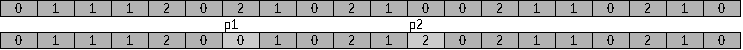
\includegraphics{Imagens/LoopMoveOperator.png}
 		\caption{Exemplo de aplicação do operador LPM. \\Fonte Autoria Própria}
 		\label{fig:loopMoveOperator}
 	\end{figure}
 	
 	\item \textit{Opposite Mutation} (OM): Esta heurística troca as direções, para direção oposta, de uma sequência de genes entre dois genes $(i,j)$ selecionados de maneira aleatória. A direção 0 ($F$) não possui oposta, portanto é mantida. Para exemplificar, suponha esta solução hipotética para uma sequência de 5 aminoácidos: $\{0,1,2,1,2\}$. Ela se tornaria $\{0,2,1,2,1\}$. A figura \ref{fig:oppositeMutation} apresenta um exemplo da aplicação do operador OM.
 	
 	
 	\begin{figure}[!htb]
 		\centering
 		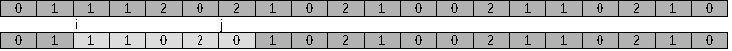
\includegraphics{Imagens/OppositeMutation.png}
 		\caption{Exemplo de aplicação do operador OM. \\Fonte Autoria Própria}
 		\label{fig:oppositeMutation}
 	\end{figure}
 	
 	
 	
 \end{itemize} 



 Este capítulo está divido em duas seções para melhor apresentar ambas as estratégias propostas nesta dissertação . A seção \ref{sec:aemos} apresenta a estratégia multi objetiva onde foi utilizada dois algoritmos evolucionários, do estado da arte de otimização multi objetiva. Já a seção  \ref{sec:eghypdp} irá apresentar o design automático de heurísticas de alto nível para um \textit{framework} hiper heurístico para resolver o PDP.
 


\section{AEMOs aplicados ao PDP}
\label{sec:aeoms}

Esta abordagem utiliza uma modelagem multi-objetiva para PDP baseado no estudo desenvolvido por \cite{gabriel2012algoritmos}. Onde o primeiro objetivo trata de maximizar a quantidade de contatos topológicos das estruturas de proteínas e o segundo de minimizar a máxima distância euclidiana entre os aminoácidos. 

Duas abordagens multi-objetivas foram desenvolvidas neste capítulo, utilizando os AEMOs (NSGAII e IBEA) descritos no capítulo \ref{cap:Referencial Teórico}. A primeira abordagem consistiu em aplicar os algoritmo IBEA and NSGAII utilizando suas versões padrão. Nesta abordagem os operadores genéticos (cruzamento e mutação) são fixos com: \textit{Single Point Crossover (1x)} and \textit{Bit Flip Mutation (BM)}. Esta foi a combinação que obteve os melhores resultados em experimentos preliminares. No caso da segunda abordagem, o IBEA e NSGAII foram modificados com objetivo de aprimorar os resultados em relação às versões padrões. Duas modificações foram propostas e serão descritas abaixo:

 
 \begin{itemize}
 		
		\item \textit{Pool} de operadores: O uso de operadores fixos geralmente não conseguem guiar a busca para regiões promissoras. Com objetivo de aprimorar os AEMOs, um \textit{pool} de operadores foi desenvolvido. Os operadores que compõem \textit{pool} foram selecionados de estudos anteriores e foram apresentados no início deste capítulo. A cada operação de cruzamento e mutação os operadores são selecionados de maneira aleatória a partir do \textit{pool}. Os operadores são sempre executados independente de probabilidades conforme a versão padrão dos algoritmos. 
	
		
		\item Inicialização via \textit{backtracking}: Tradicionalmente, a população inicial é gerada de maneira aleatória no caso dos algoritmos NSGAII e IBEA. Este tipo de inicialização tem grande potencial de gerar muitas soluções inválidas ao  modelo HP-2D. Soluções que não sejam \textit{self-avoiding walk} (SAW) são consideradas inválidas pois dois ou mais aminoácidos estariam ocupando a mesma posição no espaço. Se a população for integralmente gerada de maneira aleatória os algoritmos de otimização perdem um tempo considerável avaliando soluções inválidas. Para evitar este problema uma estratégia de \textit{backtracking} pode ser utilizada. A estratégia de inicialização com \textit{backtracking} irá começar posicionando o primeiro aminoácido na posição 0,0. Para posicionar o próximo aminoácido, um movimento é selecionado de maneira aleatória. Caso o movimento cause uma colisão, este movimento será marcado como uma má escolha e um novo movimento é selecionado aleatoriamente (do conjunto que restou sem os movimentos marcados como más escolhas). Caso todos os movimentos estejam marcados como má escolha, a estratégia de \textit{backtracking} irá retornar de maneira recursiva para o aminoácido anterior e marcar a escolha em questão como uma má escolha. A estratégia de \textit{backtracking} termina quando gerar uma conformação que não possua colisões. Entretanto, a inicialização via \textit{backtracking} é computacionalmente custosa. Dessa maneira, apenas 20\% da população inicial foi inicializada utilizando esta estratégia.

\end{itemize}

Portanto 4 algoritmos foram implementados (IBEA, NSGAII, M\_IBEA e M\_NSGAII) foram propostos para avaliar a abordagem multi objetiva para o PDP simplificado.


\subsection{Funções Objetivo}


\begin{itemize}
	\item \textbf{Valor de Energia}: Este é o objetivo principal e sua responsabilidade é avaliar o valor de energia associado com as possíveis conformações codificadas pelos cromossomos. O objetivo é minimizar o valor de energia, o qual, é calculado conforme descrito no capítulo \ref{cap:pdp}. Este objetivo guia a busca na direção onde os valores energia associados com as estruturas de proteínas sejam mínimos. Dessa maneira, obtendo conformações mais próximas ao estado nativo das estruturas de proteínas.

    \item \textbf{Distância euclideana entre os resíduos mais distantes}: Este é um objetivo secundário inspirado pelo estudo desenvolvido por \cite{gabriel2012algoritmos}. A motivação por de trás deste objetivo é que estruturas mais compactas tendem a possuir mais contatos hidrofóbicos, oque resultaria em um valor menor de energia. A distância entre os resíduos é calculada utilizando a distância euclidiana.
   
\end{itemize}

Geralmente para avaliar e comparar a performance dos AEMOs, indicadores de qualidade são utilizados. Neste estudo o indicador \textit{hypervolume} foi utilizado. Este indicador considera o volume do espaço de busca dominado pela fronteira conhecida de Pareto obtida por um algoritmo \cite{zitzler2003performance}. Um maior valor de \textit{hypervolume} significa maior qualidade na cobertura do que um algoritmo com valor inferior.

Os 4 algoritmos foram implementados utilizando a arquitetura \textit{open source} disponível no \textit{framework} jMetal. A arquitetura do jMetal é de fácil extensão e possui uma ativa comunidade.


\section{EGHyPDP}
\label{sec:eghypdp}

Esta abordagem é baseada no trabalho desenvolvido por \cite{sabar2015automatic}, o qual  utilizou GEP (\textit{gene expression programming}) com objetivo de gerar, de maneira \textit{online}, os componentes de um \textit{framework} hiper-heurístico para diversos domínios de problemas. Os testes de generalidade realizados, utilizando os 6 domínios providos pelo \textit{framework} hiper-heurístico HyFlex, apresentaram bons resultados em relação às outras estratégias hiper-heurísticas do estado da arte. Nesta proposta pretende-se utilizar EG ao invés de GEP e aplicar ao PDP simplificado utilizando o modelo HP-2D. Da mesma maneira que a abordagem que utilizou  AEMOs a representação de coordenadas relativas descrita na subseção \ref{subsubsection:modeloHP}, será utilizada. Como mencionado anteriormente, um \textit{framework} hiper-heurístico possui dois níveis: alto (\textit{high-level heuristics}) e baixo (\textit{low-level heuristics}). Nesta proposta as heurísticas de alto nível são compostas por: um mecanismo de seleção e um critério de aceitação. Já as heurísticas de baixo nível consistem em um conjunto de heurísticas, selecionadas de estudos anteriores, um mecanismo de memória e uma função de \textit{fitness}. 

\section{Heurísticas de alto nível}
\label{sec:highlevelheuristics}
Esta abordagem  foi desenvolvida para gera de maneria \textit{offline} os componentes de uma heurística de alto nível (mecanismo de seleção e critério de aceitação) para um \textit{framework} hiper-heurístico. A figura \ref{fig:proposedFramework} apresenta a estrutura geral do EGHyPDP. 

\begin{figure}[!htb]
	\centering
	\includegraphics[scale=.98]{Imagens/proposedFramework.png}
	\caption{ \textit{Estrutura geral do EGHyPDP.} \\ Fonte: Adaptado de \cite{sabar2015automatic}}
	\label{fig:proposedFramework}
\end{figure}


Heurísticas de alto nível geralmente levam em consideração uma ou mais informações referentes ao histórico das aplicações das heurísticas de baixo nível para tomar suas decisões. Tradicionalmente, informações tais como desempenho (capacidade de melhorar soluções), tempo (desde a última aplicação de uma dada heurística) e intervalo de confiança (no caso de estratégias que utilizam MAB) são utilizadas como base de conhecimento. \cite{sabar2015automatic} propõem a utilização de vários critérios para avaliar as heurísticas de baixo nível. A razão disto se dá pelo fato de que cada critério irá favorecer a seleção de uma heurística de baixo nível a partir de um aspecto diferente. Por exemplo, algumas heurísticas de baixo nível podem ter bom desempenho apenas no início da busca, enquanto outras podem obter melhores resultados apenas ao final. Estes critérios propostos por \cite{sabar2015automatic} contém estatísticas referente à aplicações das heurísticas de baixo nível e são genéricos o suficiente para serem aplicados ao PDP. Os critérios propostos por Sabar et al. \cite{sabar2015automatic} são detalhados em seguida:


\begin{itemize}
	\item RC (\textit{Reward Credit}): Representa a recompensa que uma determinada heurística de baixo nível deve receber baseado no seu desempenho durante o processo de busca. Quando a i-ésima heurística é aplicada, a melhoria para a solução é computada. O cálculo da melhoria é dado por: $M(i) = (|f1 -f2|/f1) *100$ se $f2$< $f1$, onde $f1$ é a qualidade da solução corrente e $f2$ é a qualidade da solução resultante após a aplicação da i-ésima heurística. 
	A melhoria obtida é salva em uma janela deslizante (FIFO) de tamanho W. O crédito de qualquer heurística de baixo nível é então atribuído como o máximo valor na janela deslizante correspondente. A ideia por trás deste critério é: heurísticas de baixo nível que não são usadas com frequência mas que alteram a solução com grandes melhorias tendem a ter mais preferência do que aquelas que geram pequenas melhorias. Portanto as heurísticas que trazem frequentes, mas pequenas melhorias irão ter menos probabilidade de serem selecionadas.
	\item $C_{best}$: Número de vezes que a i-ésima heurística de baixo nível atualizou a melhor solução conhecida. Este critério favorece as heurísticas de baixo nível que obtiveram êxito em melhorar a melhor solução conhecida até o momento. Este critério é útil para sistematicamente melhorar o atual mínimo local.
	\item $C_{current}$: Número de vezes que a i-ésima heurística de baixo nível atualizou a solução atual. Este critério favorece as heurísticas de baixo nível que obtém êxito em atualizar a solução corrente. Este critério serve para deixar a busca concentrada próxima à solução corrente.
	\item $C_{accept}$: Número de vezes que a solução gerada pela i-ésima heurística de baixo nível foi aceita pelo critério de aceitação. Irá favorecer heurísticas de baixo nível que podem ajudar a escapar de um mínimo local.
	\item $C_{ava}$: A média de melhorias anteriores da i-ésima heurística de baixo nível durante o progresso da busca. Este critério favorece heurísticas de baixo nível que realizaram grandes melhorias em média.
	\item $C_r$: O número de vezes que a i-ésima heurística de baixo nível foi classificada como primeira.  
\end{itemize} 

Da mesma maneira \cite{sabar2015automatic} propõem o uso de dados referentes ao histórico de aplicações das heurísticas de baixo nível para compor critérios de aceitação que irão definir limites para aceitar soluções com qualidade inferior. Dessa forma, um conjunto de fatores também foi proposto e será detalhado em seguida:


\begin{itemize}
	\item Delta: A diferença da qualidade entre a solução corrente e a solução descendente.
	\item PF: A qualidade da solução anterior.
	\item CF: A qualidade da solução atual.
	\item CI: Iteração corrente.
	\item TI: Número de iterações.
\end{itemize}


Utilizando estes dados estatísticos e um conjunto de funções matemáticas simples, tais como soma, subtração, multiplicação e divisão, uma gramática foi desenvolvida para suportar a geração das heurísticas de alto nível. A gramática desenvolvida para gerar mecanismos de seleção e critérios de aceitação é apresentada na Gramática \ref{grammar:proposedGrammar}. 

Para inicializar os dados dos terminais: todas as heurísicas foram executadas uma vez e os dados para cada terminal foi calculado. Toda iteração seguinte irá atualizar os dados dos terminais e essas informações são utilizadas durante a busca.

 \begin{Grammar}
 	\begin{grammar}
 		<hh-selection> ::= <selection-mechanism> <acceptance-criterion> 
 		
 		<selection-mechanism> :==  <selection-terminal>   
 		\alt <selection-mechanism> <math-function> <selection-mechanism> 
 		\alt (<selection-mechanism> <math-function> <selection-mechanism>) 
 		
 		<selection-terminal> :== 
 		RC 
 		| Cbest 
 		| Ccurrent 
 		| Caccept 
 		| Cava 
 		| Cr
 		
 		<math-function> :== + 
 		| - 
 		| * 
 		| \%
 		
 		<acceptance-criterion> ::== <acceptance-terminal> 
 		\alt <acceptance-criterion> <math-function>
 		<acceptance-criterion>
 		\alt (<acceptance-criterion>  <math-function> <acceptance-criterion>) 
 		
 		<acceptance-terminal> :== PF | CF | CI | TI
 		
 		%	<acceptance-function> :== + | - | * | \% | $e^x$
 		
 		
 	\end{grammar}
 	\caption{Gramática definida para gerar  heurísticas de alto nível}
 	\label{grammar:proposedGrammar}
 \end{Grammar}
 
 
  
  O conjunto de funções matemáticas para combinar de diferentes maneiras os dados históricos das aplicações das heurísticas de baixo nível é apresentado abaixo:
  
  \begin{itemize}
  	\item +: Adiciona as duas entradas.
  	\item -: Subtrai a segunda entrada da primeira.
  	\item *: Multiplica as duas entradas.
  	\item \%: Divisão protegida, isto é, se o denominador for 0, o altera para 0,001.
  \end{itemize}
  
  
  Utilizando a Gramática \ref{grammar:proposedGrammar} e vetores de inteiros é possível gerar heurísticas de alto nível. Os conjuntos terminais da gramática apresentam estatísticas sobre as heurísticas de baixo nível e estas são a matéria-prima para a construção dos componentes das heurísticas de alto nível de um \textit{framework} hiper-heurístico. 
  
  

  
  O próximo passo consiste em evoluir uma população de vetores de inteiro utilizando o processo evolutivo descrito na subseção 
  \ref{subsubsection:EvolucaoGramatical}. %A figura BLAH apresenta o processo geral da evolução gramatical proposta.
  
  
  \subsection{Função de \textit{Fitness}}
  \label{sub:funcfitness}
  
  
  	%TODO: escrever na metodologia sobre a funao de fitness escrever uma funcao bunitinha 
  	
 Com objetivo de avaliar os indivíduos gerados durante a busca, uma função de \textit{fitness} foi desenvolvida. A função executa a heurística de alto nível, representada por um dado indivíduo, em 3 instâncias aleatórias de um total de 11 selecionadas dos estudos anteriores. Para cada instância a heuristíca de alto nível foi executada com um tempo máximo de 30 minutos e o retorno é a melhor solução para o PDP simplificado com o modelo HP-2D. O valor de \textit{fitness} associado com a solução retornada é então normalizado entre 0 e 1. O \textit{fitness} de um indivíduo, da EG, consiste na soma das saídas das execuções com cada uma das 3 instâncias. Dessa maneira, o melhor valor possível é 3 e o pior é 0. A razão de executar a heurística de alto nível (indivíduo) com 3 instâncias é que treinar a EG com menos instâncias não seria suficiente para obter bons resultados em várias instâncias na fase de validação. 
 
% 
%\begin{equation}
% 	\sum_{i = 0}^{n}E(c_i)
% \end{equation}
%
%\noindent onde $ c $ é o conjunto de instâncias selecionadas de maneira aleatória no inicio do processo da EGHyPDP, sendo que o tamanho máximo, $ n $ foi definido como três.
 
 
 
   


  
  \subsection{Critério de Parada}
  \label{sub:criterioParada}
  
  Para terminar o processo da EG um número máximo de iterações que não obtêm melhora será utilizado como condição de parada. Note que este critério de parada é referente à parada do processo da EG e não das execuções dos indivíduos dentro do \textit{framework} hiper-heurístico, que ocorrem durante o progresso da EG. 
  
  
  \section{Heurísticas de baixo nível}
  
  Nas heurísticas de baixo nível o EGHyPDP possui 2 componentes principais: um conjunto de heurísticas de baixo nível e um mecanismo de memória.
  
  \subsection{Conjunto de heurísticas de baixo nível}
  O conjunto de heurísticas de baixo nível foi desenvolvido baseado estudos anteriores e foi apresentados no início deste capítulo.
  



\section{Processo geral do EGHyPDP} 

As principais etapas da EGHyPDP proposta serão apresentadas nesta seção.
Inicialmente uma população de indivíduos (heurísticas de alto nível: mecanismos de seleção e critérios de aceitação) é gerada conforme o procedimento que será descrito posteriormente nesta seção. O \textit{fitness} da população é calculado inserindo os indivíduos em um \textit{framework} hiper-heurístico e o executando com 3 instâncias por 30 minutos. E de maneira iterativa selecionar indivíduos pais e aplicar os operadores de cruzamento, \textit{prune}, mutação, e \textit{duplicate} para gerar descendentes. Posteriormente, estes indivíduos são submetidos ao processo de avaliação descrito na subseção \ref{sub:funcfitness}.

%Para avaliar os indivíduos gerados, os seguintes passos são executados:


O processo da EGHyPDP irá parar apenas quando o critério de parada discutido na subseção \ref{sub:criterioParada} for atingido e será retornado o indivíduo (heurística de alto nível) que possuir o maior valor de \textit{fitness}. Também será retornada a solução ao PDP que tiver maior qualidade no mecanismo de memória.



\subsection{Mecanismo de Memória}
\label{sub:MecanismoDeMemoria}

A maioria dos \textit{frameworks} hiper-heurísticos propostos na literatura operam sobre uma única solução \cite{chakhlevitch2008hyperheuristics, burke2013hyper}. Blum et al. \cite{blum2011hybrid} menciona que utilizar uma única solução pode restringir a capacidade de explorar complexos espaços de busca e com alta variância de características. Dessa maneira,  \cite{sabar2015automatic} propôs uma abordagem que utiliza um mecanismo de memória, assim como  \cite{talbi2006cosearch}, o qual contém um conjunto de soluções com alta qualidade e diversificadas, atualizado durante o progresso da busca. Nesta proposta o mecanismo de memória tem a responsabilidade de armazenar soluções para o problema PDP utilizando a representação de coordenadas relativas para o modelo HP-2D. 

\subsubsection{Inicialização do Mecanismo de Memória}

Tradicionalmente algoritmos evolutivos inicializam suas populações iniciais de maneira aleatória, por conta disto  muitas soluções inválidas ao modelo HP, são geradas na inicialização. Isto geralmente  ocasiona perda de tempo de processamento, por conta da grande quantidade de conformações inválidas antes que bons resultados sejam obtidos. Diante disto, \cite{benitez2015algoritmo} propôs uma estratégia especializada de inicialização. A população de seu algoritmo genético, é dividia em duas partes. Uma gerada aleatoriamente, com indivíduos que potencialmente possuem colisões. E uma segunda parte onde todos os indivíduos são livres de colisões. Uma configuração é utilizada para definir a proporção entre as duas partes da população inicial. Para garantir que os indivíduos não possuam colisões, uma estratégia de \textit{backtracking} deve ser utilizada. Nesta abordagem, a mesma estratégia de inicialização via \textit{backtracking }, descrita  na seção \ref{sec:aeoms} foi implementada.





%As possíveis conformações podem ser representadas por um caminho em um grafo orientado estruturado como uma árvore. Consequentemente, cada nó da árvore representa uma solução candidata parcial $c$, desde o primeiro aminoácido até o último sendo considerado. Portanto, um caminho até um nó folha representa uma conformação completa. As arestas do grafo representam o movimento de cada aminoácido relativo a seu predecessor.



\subsubsection{Atualização do Mecanismo de Memória}
Para cada indivíduo (heurística de alto nível) será selecionada de maneira aleatória uma solução do mecanismo de memória e a busca irá iniciar em torno desta solução, quando o \text{framework} hiper-heurístico atingir o seu número máximo de iterações a solução final tem que ser avaliada para verificar sua qualidade e diversidade. A qualidade de uma solução para o PDP utilizando o modelo HP é inversamente proporcional à quantidade de interações entre aminoácidos hidrofóbicos. Portanto a qualidade de uma solução é dada pela quantidade de iterações H-H multiplicada por -1, conforme descrito na subseção \ref{subsubsection:modeloHP}.  As soluções geradas que tiverem a qualidade maior que todas as soluções contidas no mecanismo de memória substituirão a solução que tiver menor similaridade segundo a distância de  \cite{hamming1950error}. Se a qualidade de uma solução gerada não for maior que todas as soluções, mas melhor em relação a um sub-conjunto do mecanismo de memória, esta substituirá a solução que tiver menor qualidade e menor similaridade do sub-conjunto. E por fim se a qualidade da solução gerada for pior que todas contidas no mecanismo de memória, esta é descartada. A similaridade é considerada a fim de manter a diversidade entre as soluções.  



\section{Considerações Finais}
\label{Metodologia:ConsideracoesFinais}

Neste capítulo foram discutidos os principais aspectos relativos à duas estratégias propostas nesta dissertação. Inicialmente, foi discutido sobre a aplicação de AEMOs e em seguida o EGHyPDP foi apresentado. A representação relativa foi utilizada para codificar as soluções para ambas as estratégias. O conjunto de heurísticas de baixo nível, utilizado em ambas abordagens, também foi apresentado. No caso dos AEMOs 4 versões de algoritmos foram apresentadas. As funções objetivas também foram discutidas. Duas adaptacões foram propostas que consistiram em adicionar um \textit{pool} de operadores para tornar os AEMOs mais adpatativos e a inicialização via \textit{backtracking}. Para aplicar o EGHyPDP com objetivo de gerar heurísticas de alto nível de um \text{framework} hiper-heurístico para o PDP simplicado, uma  gramática foi desenvolvida. Também foi apresentado um conjunto de terminais referente ao histórico das aplicações das heurísticas de baixo nível. Funções matemáticas simples compõem a gramática e combinadas com os dados estatísticos diferentes heurísticas de alto nível foram geradas. Posteriormente, a função de \textit{fitness} avalia estas heurística executando o \textit{framework} composto por tais trés vezes em três instâncias distintas selecionadas de maneira aleatória.
 
 O próximo capítulo apresenta os experimentos realizados afim de avaliar o desempenho das abordagens aqui propostas.



